\subsection{Bioinformatics Analysis of Human IFITs} \label{subsec:Bioinformatics Analysis of Human IFITs}
lorem ipsum

\subsubsection{Validation Proteomics Data}

\begin{figure}
    \centering
    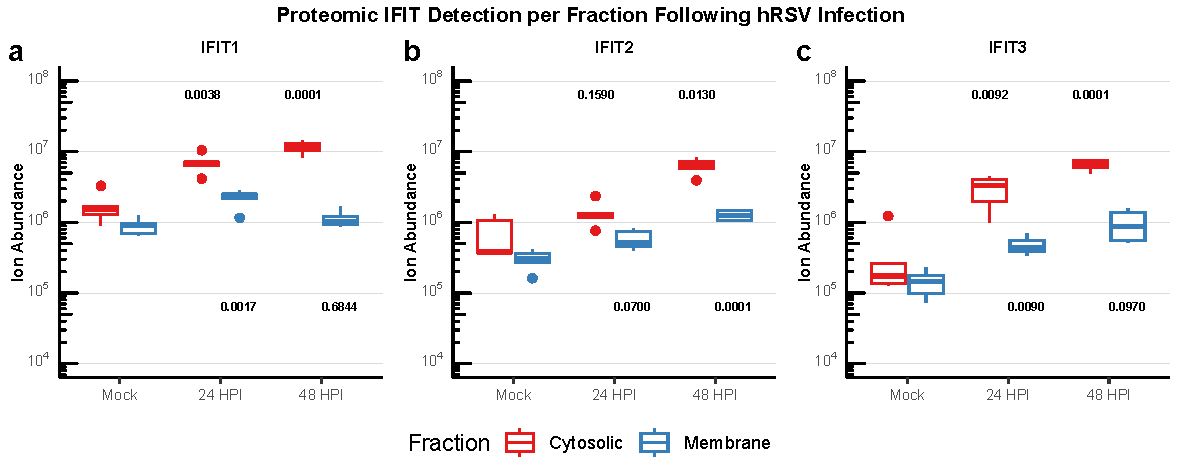
\includegraphics[width=1\linewidth]{08. Chapter 3/Figs/01. Human/01. merged_proteomics.pdf}
    \caption[Human IFIT proteins detected per fraction.]{\textbf{Human IFIT proteins detected per fraction.} Analysis of summed peptide intensities of (a) hIFIT1, (b) hIFIT2, and (c) hIFIT3 detected per either cytosolic or membrane fractions of A549 cells which were either mock-infected or infected with hRSV MOI 1 for either 24 or 48 hours. There were no hits for IFIT5. This data is from a proteomic study, published in \cite{Jobe2023ViralCondensates}. Samples are composed of biological quintuplicates. Numeric values signify the p-values compared to the respective mock, i.e. top numbers for cytosolic fraction, bottom for membrane fraction.}
    \label{fig:Human IFIT proteomics.}
\end{figure}

To conclude the assessment of human IFIT responses to human RSV, I was kindly provided with a quantitative mass spectrometry dataset of human IFITs detected in either cytosolic or membrane fraction of either mock-infected or cells infected with human RSV at MOI 1, processed 24 or 48 HPI. This dataset was provided by Dr Kelly and Dr Jobe from the Pirbright Institute and its findings have now been published (\cite{Jobe2023ViralCondensates}). Quintuplicates of cytosolic and membrane fractions were isolated by in-gel digestion and analysed by label-free quantitative mass spectrometry. Normalised and log-transformed ion abundance data for hIFIT1, hIFIT2, and hIFIT3 can be seen in Figure \ref{fig:Human IFIT proteomics.}. hIFIT1 cytoplasmic and hIFIT2 membrane datasets had normal distributions and equal variances, while all the others displayed normal distributions with non-equal variances. Human IFIT5 did not yield any hits and thus was excluded from the analysis and we can conclude that its proteome is not drastically changed by hRSV infection, which is in line with our qPCR data. hIFIT1 is the most basally abundant, followed by hIFIT2 and hIFIT3. The basal abundance of hIFITs is around equal between the fractions. The infection at 24 HPI causes increased abundance of all hIFITs in all fractions, more specifically hIFIT1 increased 5x in the cytosolic fraction and 1.3x in membrane fraction; hIFIT2 increased 4x in cytosolic and 2x in membrane fractions; and hIFIT3 increased relatively the most by 13.5x in the cytosolic fraction and 3x in the membrane fraction. The highest total abundance at 24 HPI was still hIFIT1. At 48 HPI we can observe a further increase in abundance for all other than hIFIT1 in membrane fraction which decreased to mock levels. In more detail, hIFIT1 in cytosolic fraction increased further 2x; hIFIT2 increased further 5x in cytosolic and 4x in membrane fraction; and hIFIT3 further increased 3x in cytosolic fraction and 2.5x in membrane fraction. These data together validate our qPCR results seen in Figure \ref{fig:A549 response to hRSV timepoints} and Figure \ref{fig:The effect of ultra-purification, UV-inactivation and INFR inhibition on hIFIT induction following hRSV infection in A549} and highlight the differential spatio-temporal expression dynamics of human IFITs.

normal unequal - 2c 3c 3m

normal euqal - 1c 1m 2m 


\subsubsection{Meta-Analysis}
lorem ipsum

\subsubsection{Summary}
lorem ipsum
